\section{Frontend}

\subsection{AngularJS}

AngularJS ist ein JavaScript Framework. Die wichtigste Eigenschaft ist, dass es HTML-Elemente um zusätzliche Attribute erweitert. Die zwei wahrscheinlich wichtigsten und bezeichnensten davon sind \verb|ng-model| und \verb|ng-bind|. \verb|ng-bind| bindet Variablen vom JavaScript Code an HTML-Element Inhalte. Die von \verb|ng-bind| hergestellte Datenbindung geht aber nur in eine Richtung. \verb|ng-model| bindet Variablen von der HTML-View an Variablen im JavaScript Code. Im Gegensatz zu \verb|ng-bind| stellt \verb|ng-model| jedoch eine Datenbindung her, die in beide Richtungen funktioniert. Das bedeutet, dass wenn sich eine Variable im  Code ändert, ändern sich auch die verbundenen Anzeigeelemente und umgekehrt.

\subsubsection{Promises}
AngularJS erweitert nicht nur die View-Elemente des Frontends, sondern es stellt auch viele sehr nützliche JavaScript Funktionen und Erweiterungen zur Verfügung. Eine davon sind Promises. Promises stellen ein sehr gutes Werkzeug dar, um dem JavaScript Callback-Chaos Herr zu werden. Das Konzept basiert darauf, dass ein Promise eine \verb|.then(fkt_success, fkt_fail)| Methode besitzt, die aufgerufen wird, sobald die Aufgaben im Promise erledigt wurden. \verb|.then()| bekommt zwei Parameter: eine Funktion, die im Erfolgsfall, eine die im Fehlerfall ausgeführt werden soll. Das wichtige ist nun, dass jeder Promise wieder einen Promise als Returnwert besitzt, sofern es erwünscht wird, dass nach den Operationen im 1. Promise neue Operationen ausgeführt werden sollen. Der neue Promise besitzt natürlich wieder eine \verb|.then()| Methode. Promises lösen so einige Unannehmlichkeiten in Javascript die vor allem durch die Verwendung und Verschachtelung von Callbacks entstehen\footnote{\url{https://angularjs.de/buecher/angularjs-buch/angularjs-promises}}:

\begin{itemize}
	\item Übersichtlichkeit - Pyramids of Doom
	\item Fehlerbehandlung - Abfangen und Korrektur von Fehlern
	\item Parallelität - Synchronisation mehrerer Asynchronitäten
	\item Vermischung von Verantwortlichkeiten
\end{itemize}

\subsection{Tabs}
Tabs sind eine sehr gute Möglichkeit, Weboberflächen Übersichtlich, und gut navigierbar zu gestalten. Das Framework Bootstrap stellt hierzu schon CSS-Klassen zur Verfügung, mit denen sich Tabs leicht erstellen lassen. In Verbindung mit Angular kann so sehr gut eine leicht zu erweitende Tab-Umgebung eingerichtet werden. Im JavaScript Teil des Frontends braucht lediglich eine Zeile bei der Angular-Controller initialisierung hinzugefügt werden:

\scriptsize
\begin{lstlisting}[language=Javascript]
$scope.tabs.push({label: "MyTab", execute: test, fkt_params: "test_string"});
\end{lstlisting}
\normalsize

Dadurch wird auf der HTML-Seite automatisch ein neuer Tab mit dem Namen 'MyTab' hinzugefügt. \verb|$scope| wird hier für alle JavaScript-Elemente verwendet, die im AngularJS-Scope verfügbar sind, d.h. Datenelemente sind, die sowohl im HTML-Teil (z.B. durch \verb|ng-model|) als auch im JavaScript Teil (Funktionen, Variablen) verwendet werden. Außerdem kann jedem Tab eigens eine Funktion zugewiesen werden, die beim Wechsel auf diesen Tab mit den angegebenen Parametern ausgeführt wird. 

In Code-Segment \ref{cs:tabs_html} ist zu sehen, wie die Tabs in der HTML-View umgesetzt werden. Zuerst wird mit \verb|<ul class="nav nav-tabs">| eine Navigations-Tab Umgebung geöffnet. Darin kommt der wahrscheinlich wichtigste AngularJS Befehl zur Verwendung: \verb|ng-repeat|. \verb|ng-repeat| erzeugt eine Schleife, die den HTML-Tag in dem sie verwendet wird (hier \verb|<li>|) für alle Elemente im Objekt das nach dem Schlüsselwort \verb|in| kommt (hier \verb|tabs|) wiederholt wird. Das Objekt \verb|tabs| ist genau das Selbe, dass vorher im JavaScript-Code mit \verb|$scope.tabs| erweitert wurde. Der Content eines Tabs kann dann bliebig befüllt werden. Dazu muss nur noch ein eigenes \verb|<div>| Element mit dem gewünschten Inhalt hinzugefügt werden. Ein Muster dafür ist auch im Code-Segment \ref{cs:tabs_html} zu sehen. Hier ist auch noch zu sehen, dass der neu erstellte \verb|<div>|-Container mit der Angula Direktive \verb|ng-show| versehen ist. Dadurch kann die Bedingung festgelegt werden, dass der \verb|<div>|-Container nur dann sichtbar sein soll, wenn die Bedingung danach erfüllt ist.

\scriptsize
\begin{lstlisting}[caption=index.html, label=cs:tabs_html, language=HTML]
<!------- tab-creation -------->
<ul class="nav nav-tabs">
	<li class="{active:wa_ctrl.tab === $index}" ng-repeat="tab in tabs">
		<a href ng-click="wa_ctrl.selectTab(tab.label)">{{tab.label}}</a></li>
	</li>
</ul>

<!------- lines omitted -------->

<!------- own tab content -------->
<div class="wa_ctrl"  ng-show="wa_ctrl.isSelected('MyTab')">
	<p> MyTab </p>
</div>
\end{lstlisting}
\normalsize

Ein sehr guter Nebeneffekt dieses Seiten-Design ist, dass sich alles auf einer einzigen HTML-Seite abspielt. Es handelt sich dabei um ein Single-Page-Layout. Dieses Entwurfsmuster hat einige wesentliche Vorteile, auf die hier aber nicht näher im Detail eingegangen wird. 

Wichtig zu erwähnen ist auch noch, dass das Backend eine Initialisierungs-URL zur Verfügung stellt, die eine JSON-Liste mit allen Verfügbaren Entitäten und den dazugehörigen, in den Controllern festgelegten mappings, Referenz URL's. Dadurch wird automatisch beim Öffnen der Seite für jede Verfügbare Entität ein Tab erstellt, der das Bearbeiten und Anzeigen der Entitäten ermöglicht.

\subsection{Eingabeform}

Nun ist es natürlich wünschenswert, in jedem Entity-Tab die Möglichkeit zu haben, ein neues Objekt der Entität zur Datenbank hinzuzufügen. Aus diesem Grund wurde eine Form erstellt, die genau das ermöglicht. Über den zur Entität gehörenden GET-Request wird wie schon vorher erläutert ein JSON-Objekt das die Struktur der gewählten Entität enthält. Aufgrund dieses Objektes ist es möglich, für jedes Attribut der Entität ein passendes Eingabeelement zu erzeugen. So wird zum Beispiel für die Telefonnummer einer Person ein Textfeld erzeugt da es sich um eine Variable vom Typ \verb|String|, für das Attribut Anwesenheit aber eine Checkbox, da es vom Typ \verb|Boolean| ist. Nun bleibt noch die Frage nach den Fremdschlüsseln offen. Dieses Problem wird im selben Abschnitt gelöst. Das alle verfügbaren Fremdschlüssel sich ja schon im empfangenen JSON-Objekt befinden, können diese ganz einfach über eine Drop-Down Leiste in die Eingabeform integriert werden. Ein Ausschnitt dazu ist in Abbildung \ref{fig:input_form} zu sehen. Mit diesem Konzept ist es sehr einfach möglich dynamisch eine sehr gute Eingabeform zu erstellen.

\scriptsize
\begin{lstlisting}[caption=Erstellung der Eingabeform in index.html, label=cs:input_form, language=HTML]
<tr ng-show="new_entry_visible">
	<td ng-repeat="attribute in attributes">
		<!-- choose whether to display a "normal" input type, or a dropdown-list-->
		<input ng-if="input_types[attribute] != 'select'" type="{{input_types[attribute]}}" name="{{attribute}}" ng-model="new_db_object[attribute]" />
		
		<select ng-if="input_types[attribute] == 'select'" ng-model ="new_db_object[attribute]">
			<option ng-repeat="id in foreign_ids[attribute]" value="{{id}}">
			{{wa_ctrl.printObject(id)}}
			</option>
		</select>
	</td>
</tr>
\end{lstlisting}
\normalsize 

\begin{figure}[h]
\centering
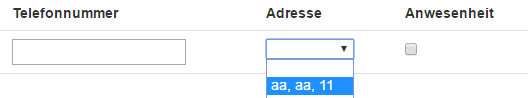
\includegraphics[width=0.7\linewidth]{4_frontend/pics/input_form}
\caption{Ausschnitt aus der Eingabeform für ein Person-Objekt}
\label{fig:input_form}
\end{figure}


\subsection{Tabellen}

Der letzte offene Punkt ist die Darstellung der bereits in der Datenbank vorhandenen Objekte. Grundsätzlich werden auch diese über den Controller der jeweiligen Entität abgefragt, und als JSON-Liste ans Frontend gesendet. Mit AngularJS können diese Daten dann dynamisch in einer Tabelle werden. Dazu ist als Vorkenntnis nur die Struktur der Daten notwendig, die sowieso schon durch die Erstellung der Eingabe-Form vorhanden ist. Die Erstellung dieser Liste ist im Code-Segment \ref{cs:input_form} zu sehen.

\scriptsize
\begin{lstlisting}[caption=index.html, label=cs:input_form, language=HTML]
<!-- row-section: object = one object (= row) of the list -->
<tr ng-repeat="object in obj_list | filter:search">
	<!-- column-section: access every property of every object -->
	<td ng-repeat="attribute in attributes">
		<!-- pretty object print if necessary  -->
		<div ng-switch on="is_foreign_id[attribute]">
			<div ng-switch-when="true">
				{{wa_ctrl.printObject(object[attribute])}}
			</div>
			<div ng-switch-default>
				{{object[attribute]}}
			</div>
		</div>
	
	</td>
	<!-- delete button-->
	<td> <button ng-click="wa_ctrl.deleteEntity($index)">Delete</button> </td>
</tr>
\end{lstlisting}
\normalsize 

\begin{figure}
\centering
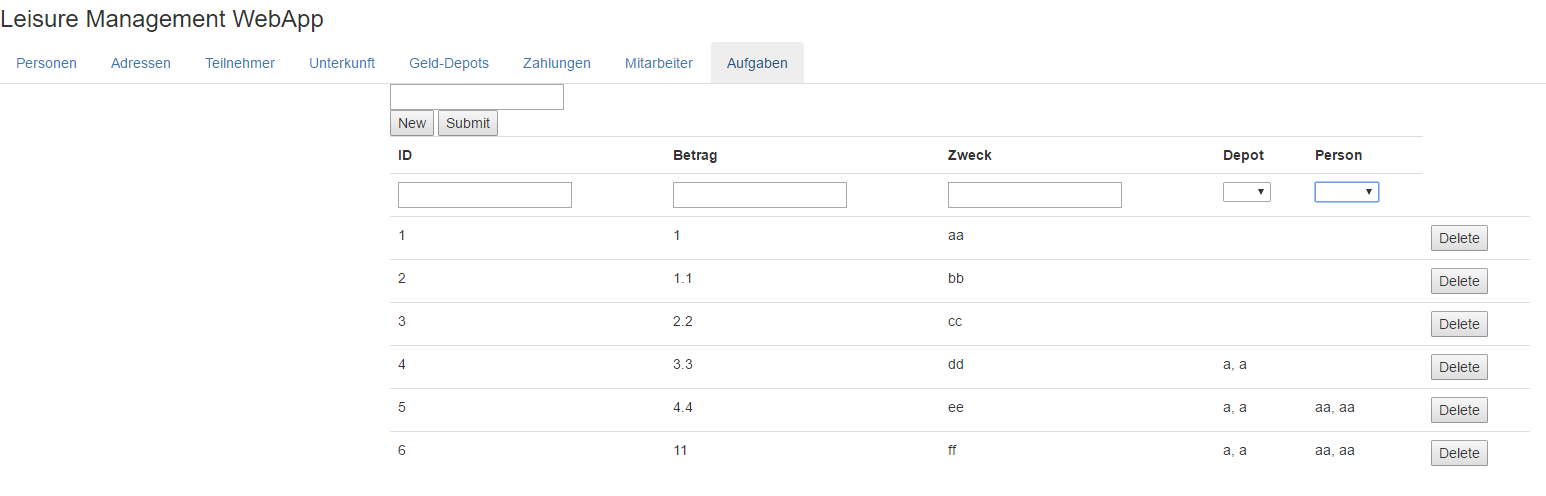
\includegraphics[width=1.4\linewidth, angle=90]{4_frontend/pics/frontend_complete}
\caption{Übersicht über das fertige Frontend, angezeigt wird der Tab für die Zahlungen}
\label{fig:frontend_complete}
\end{figure}


